\documentclass[a4paper]{article}
\usepackage{color}
\usepackage{url}
\usepackage{graphicx}
\usepackage{caption}
\usepackage[T2A]{fontenc}
\usepackage[utf8]{inputenc}
\usepackage{graphicx}
\usepackage[english,serbian]{babel}
\usepackage[unicode]{hyperref}
\usepackage{tabularx}
\usepackage{adjustbox}
\setcounter{secnumdepth}{2}
\hypersetup{colorlinks,citecolor=blue,filecolor=green,linkcolor=blue,urlcolor=blue} 

\begin{document}
\title{Sepcifikacija za projekat ClassyCrafT}


\author{Matija Radulović, Jovana Lazić\\
\small Računarski fakultet}
\maketitle


\section{Uvod}
\textit{ClassyCrafT} je aplikacija koja omogućava korisnicima da jednostavno naprave i uređuju UML dijagrame klasa. Korisniku su na raspolaganju alati pomoću kojih dodaje i povezuje objekte na radnoj površini. 

\section{Rečnik}
\begin{itemize}
    \item klasa - organizovana celina podataka i operacija nad podacima
    \item interfejs - navodi skup dostupnih operacija, nalik klasi bez atributa
    \item metod - operacija, odnosno funkcija u okviru klase
    \item atribut - polje podataka unutar klase
    \item UML dijagram klasa - standardizovan crtež simbola koji opisuje hijerarhiju klasa
    \item veza asocijacije - povezuje dve klase koje su svesne jedna druge i međusobno komuniciraju, koriste uzajamno funkcionalnosti
    \item veza agregacije - podskup gornje veze u kojem objekat jedne klase sadrži u sebi objekat druge, pritom sadržani objekat ima smisla da postoji i samostalno
    \item veza kompozicije - slično kao veza agregacije, s tim što sadržani objekat ne može postojati sam za sebe
    \item veza zavisnosti - povezuje klijentsku klasu sa pružaocem usluga koji joj nudi funkcionalnosti i od kojeg zavisi
\end{itemize}

\section{Konkurencija}

U tabeli su, radi poređenja sa ClassyCrafT aplikacijom, prikazane neke od najpopularnijih aplikacija za kreiranje UML dijagrama i funkcionalnosti koje svaka od njih implementira.

\begin{table}
\Huge
\centering
\begin{adjustbox}{width=\textwidth}
\def\arraystretch{1.8}
\begin{tabular}{ |c|c|c|c|c|c|c|c| } \hline
    & \bf{Desktop aplikacija} & \bf{Veb aplikacija}  & \bf{Lako za korišćenje} & \bf{Specijalizovano} & \bf{Besplatno} & \bf{Generisanje koda} & \bf{Stablo komponenti}  \\ \hline
 \bf{ClassCrafT} &da &ne  &ne  &da  &da &da &da  \\ \hline
 \bf{Lucid chart} &ne  &da  &da  &ne &da &ne &ne   \\ \hline
 \bf{Visual Paradigm} &da  &da  &da  &ne  &da &ne &ne   \\ \hline
 \bf{Nulab Cacoo} &ne  &da  &da  &ne  &da &ne &ne   \\ \hline
 \bf{Draw.io} &ne  &da  &ne  &ne  &da &ne &ne \\ \hline
 \bf{Gleek.io} &ne  &da  &ne  &da  &da &ne &ne  \\ \hline
 \bf{Microsoft Visio} &da  &da  &da  &da  &ne &ne &ne \\ \hline
 \bf{Astah} &da  &ne  &da  &da  &da &da &ne  \\ \hline
 \bf{ArgoUML} &da  &ne  &ne  &da  &da &da &ne  \\ \hline

\end{tabular}
\end{adjustbox}
\end{table}


\section{Korisnici}
Od korisnika se očekuje da je upoznat sa osnovnim pravilima UML standarda. Ovaj program je pre svega namenjen kao alat stručnim licima, programerima, menadžerima, projektantima, koji se bave modeliranjem i projektovanjem strukture i organizacije klasa programa. ClassyCrafT pruža grafički korisnički interfejs putem kojeg korisnik dodaje potrebne elemente za pravljenje klasnog dijagrama. 
\section{Zahtevi}
Prilikom analize domena problema utvrđene su sledeće funkcionalnosti koje bi program trebao da podrži. Zahtevi su, radi preglednosti, logički grupisani u celine, i funkcionalnostima je dat prioritet (visok, srednji nizak) u zavisnosti od neophodnosti i presudnosti datog zahteva na celokupnu upotrebljivost programa.
\subsection{Pravljenje i brisanje strukture projekta}
\subsubsection{Pravljenje i brisanje novog projekta}
Korisnik treba da bude u mogućnosti da kreira novi projekat, kao i da obriše postojeći. Prioritet je visok, rizik visok. Ukoliko korisnik slučajno obriše pogrešan projekat nema mogućnost da ga vrati, gubi sav dotadašnji rad.  
\subsubsection{Pravljenje i brisanje novog paketa}
Korisnik treba da bude u mogućnosti da kreira novi paket, kao i da obriše postojeći. Prioritet je visok, rizik visok. 
\subsubsection{Pravljenje i brisanje novog dijagrama}
Korisnik treba da bude u mogućnosti da kreira novi dijagram, kao i da obriše postojeći. Prioritet je visok, rizik visok.  
\subsubsection{Dodavanje i uklanjanje nove klase ili interfejsa}
Korisnik treba da bude u mogućnosti da kreira novu klasu i interfejs, kao i da obriše postojeće. Prioritet je visok, rizik srednji.  
\subsubsection{Dodavanje i uklanjanje metoda i atributa}
Korisnik treba da bude u mogućnosti da doda nove metode i atribute, kao i da obriše postojeće. Prioritet je visok, rizik srednji.  
\subsubsection{Dodavanje i uklanjanje veza} 
Korisnik treba da bude u mogućnosti da doda novu vezu, kao i da ukloni trenutno postojeću. Prioritet je visok, rizik srednji.  
\subsubsection{Dodavanje i uklanjanje komentara}
Korisnik treba da bude u mogućnosti da doda novi komentar, kao i da ukloni postojeći. Prioritet je srednji, rizik srednji.  
\subsection{Izmena polja}
\subsubsection{Izmena naziva projekta, paketa, dijagrama, klase}
Korisnik treba da bude u mogućnosti da modifikuje naziv već kreiranog projekta, paketa, dijagrama ili klase. Prioritet je srednji, a rizik je nizak.  
\subsubsection{Izmena naziva i tipa metoda ili atributa}
Korisnik treba da bude u mogućnosti da menja naziv, tip i vidljivost već kreirane metode odnosno atributa. Prioritet je srednji, dok je rizik nizak.  
\subsubsection{Izmena osobina i vrste veze}
Korisnik treba da bude u mogućnosti da modifikuje tip, usmerenost, kardinalnost i opcionalnost već kreirane veze. Prioritet je srednji, rizik nizak.  
\subsection{Raspoređivanje i menjanje izgleda}
\subsubsection{Promena pozicije i velicine klasa i interfejsa}
Korisnik treba da bude u mogućnosti da menja poziciju i veličinu već kreirane klase, odnosno interfejsa. Prioritet je srednji, rizik je nizak.  
\subsubsection{Promena spoja i putanje veze}
Korisnik treba da bude u mogućnosti da prespoji vezu na drugi objekat i krivuda, menja, putanju linije već kreirane veze. Prioritet je nizak, a rizik nizak. 
\subsubsection{Zumiranje i pomeranje radne površine}
Korisnik treba da bude u mogućnosti da zumira i pomera se po celokupnoj radnoj površini. Prioritet je srednji, rizik nizak.
\subsection{Alatke za rad}
\subsubsection{Kopiranje elemenata}
Korisnik treba da bude u mogućnosti da napravi kopiju već postojećeg elementa i da isti nalepi u bilo koji otvoreni dijagram. Prioritet je srednji, rizik nizak.  
\subsubsection{Istorija izmena}
Korisniku treba da bude omogućeno da poništi prethodno izvršenu radnju i vrati se u prethodno stanje. Prioritet je srednji, a rizik nizak.
\subsubsection{Selekcija elemenata}
Korisnik treba da bude u mogućnosti da odabere jedan ili više elemenata kako bi ih obeležio za primenu akcija. Prioritet je sredni, a rizik nizak.
\subsubsection{Stablo strukture projekata}
Korisnik treba da bude u mogućnosti da sa leve strane ekrana vidi sve komponmente svog projekta raspoređene u stablo. Prioritet je srednji, a rizik nizak. 
\subsection{Čuvanje projekata}
\subsubsection{Čuvanje i učitavanje projekata}
Korisnik treba da bude u mogućnosti da sačuva i učita već sačuvan projekat. Prioritet je visok, a rizik nizak.
\subsubsection{Izvoz i deljenje}
Korisniku treba da je omogućeno da dijagram podeli sa drugima u radnom, pdf, png ili nekom drugom formatu. Prioritet nizak, rizik nizak.
\subsection{Napredna pomagala}
\subsubsection{Automatsko raspoređivanje}
Korisniku treba da bude omogućeno da, nakon kreiranja i povezivanja, automatski, što preglednije, rasporedi elemente po radnoj površini. Prioritet je nizak, a rizik nizak. 
\subsubsection{Prikaz mape radne površine}
Korisnik treba da bude u mogućnosti da ima pregled celokupnog dijagrama u smanjenom prikazu na radnoj površini. Prioritet je nizak, i rizik nizak.
\subsubsection{Izvoz koda}
Korisniku treba omogućiti da iz napravljenog dijagrama generiše kostur koda klasa u jednom od podržanih programskih jezika. Prioritet nizak, rizik nizak. 
\newpage
\section{Dijagram funkcionalnosti}

\begin{figure}[h]
    \centering
    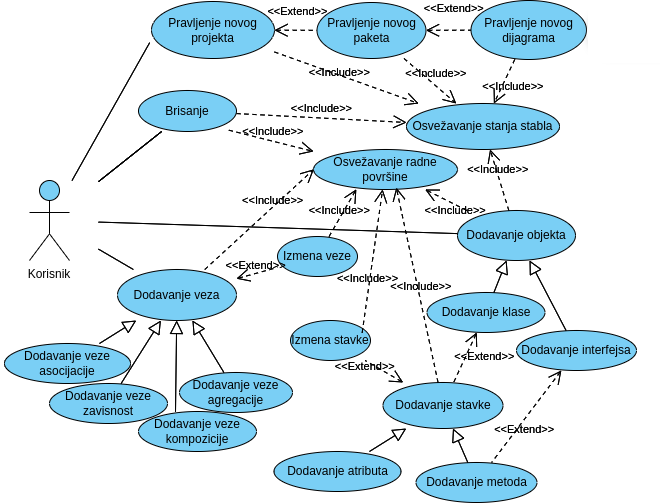
\includegraphics[width=\textwidth]{use_case_dijgram.png}
    \caption {Dijagram funcionalnosti za ClassyCrafT}
    \label{fig:enter-label}
\end{figure}

\section{Akcije korišćenja}
\subsubsection{Pravljenje novog projekta}\noindent
\textbf{Preduslov:} Nema posebnih uslova, samo je potrebno imati pokrenut program
\\ \textbf{Opis:} Klikom na odgovarajuće dugme u meniju korisnik pravi i imenuje novi projekat
\\ \textbf{Izuzetak:} Prekoračen je maksimalan broj projekata, projekat sa datim imenom već postoji
\\ \textbf{Stanje:} Nakon vršenja akcije dodaje se nov projekat u koji je moguće dodavati dalje elemente, dodat je njegov prikaz u stablu
\subsubsection{Pravljenje novog paketa}\noindent
\textbf{Preduslov:} Potrebno je da je prethodno napravljen i izabran projekat u koji želimo da dodamo paket
\\ \textbf{Opis:} Pritiskom na dugme dodaje se paket sa imenom koji unosi korisnik
\\ \textbf{Izuzetak:} Paket sa datim imenom već postoji
\\ \textbf{Stanje:} Dodat je nov paket u projekat i prikazan je u stablu
\subsubsection{Pravljenje novog dijagrama}\noindent
\textbf{Preduslov:} Napravljen je paket u koji dodajemo dijagram
\\ \textbf{Opis:} Klikom na dugme pravi se novi, prazni, dijagram 
\\ \textbf{Izuzetak:} Dijagram sa datim imenom već postoji u okviru paketa
\\ \textbf{Stanje:} Napravljen je novi dijagram na koji možemo dodavati ostale elemente
\subsubsection{Dodavanje objekta}\noindent
\textbf{Preduslov:} Izabran je i napravljen dijagram u koji želimo da dodamo objekte 
\\ \textbf{Opis:} Na odgovarajuće dugme, a potom i klikom na radnu površinu, dodaje se nova klasa odnosno interfejs na mesto izabrano pozicijom miša
\\ \textbf{Izuzetak:} Nema nikakvih izuzetaka
\\ \textbf{Stanje:} Napravljena je nova klasa odnosno interfejs, prikazana je i nalazi se u radnoj površini kao i na stablu sa leve strane
\subsubsection{Dodavanje stavke}\noindent
\textbf{Preduslov:} Postoji i izabran je odgovarajući objekat 
\\ \textbf{Opis:} Pritiskom dugmeta bira se dodavanje metode ili atributa i unose se naziv, vidljivost i tip promenljive, za metode i parametri i povratna vrednost
\\ \textbf{Izuzetak:} Pokušaj dodavanje atributa interfejsu, dodavanje metoda sa istim potpisom ili atributa sa istim nazivom, nepostojeći tip podataka
\\ \textbf{Stanje:} Dodata je nova stavka u za nju namenjen deo u okviru klase odnosno interfejsa
\subsubsection{Dodavanje veze}\noindent
\textbf{Preduslov: }Postoje barem dva napravljena objekta \\
\textbf{Opis: }Bira se tip veze pritiskom na dugme a zatim se pritiskaju dva objekta između kojih hoćemo da se napravi veza\\
\textbf{Izuzetak: }Veza tog tipa ne može da povezuje izabrane objekte, umesto drugog objekta pritisnuta je prazna površina\\ 
\textbf{Stanje: }Prikazuje se veza između odabranih objekata, usmerena od prvog ka drugom 
\subsubsection{Brisanje elemenata}\noindent
\textbf{Preduslov: }Postoji barem jedan element \\
\textbf{Opis: }Bira se dugme za brisanje, a zatim se bira element koji biva brisan \\
\textbf{Izuzetak: }Nema izuzetaka \\ 
\textbf{Stanje: }Uklanja se element sa radne površini i sa stabla ukoliko se tamo nalazi 
\subsubsection{Izmena veze}\noindent
\textbf{Preduslov: }Veza postoji i izabrana je \\
\textbf{Opis: }Bira se veza i pomoću ponuđenih dugmića menjaju se opcija vezane za usmerenost, tip i ostale karakteristike \\
\textbf{Izuzetak: }Izmenjena veza nema smisla \\ 
\textbf{Stanje: } Menja se tip i izgled veze
\subsubsection{Izmena stavke}\noindent
\textbf{Preduslov: }Postoji i izabrana je stavka \\
\textbf{Opis: }Bira se stavka i unose se izmene tipa, vidljivosti ili naziva \\
\textbf{Izuzetak: }Tip ne postoji \\ 
\textbf{Stanje: }Promenjena je stavka 
\subsubsection{Osvežavanje radne površine}\noindent
\textbf{Preduslov: }Nema preduslova \\
\textbf{Opis: }Prilikom svake izmene automatski se vrši ponovno crtanje radne površine kako bi se prikazale novonastale izmene\\
\textbf{Izuzetak: }Nema izuzetaka \\ 
\textbf{Stanje: }Prikazuje se vizualni izgled trenutnog stanja 
\subsubsection{Osvežavanje stanja stabla}\noindent
\textbf{Preduslov: }Nema preduslova \\
\textbf{Opis: }Prilikom svakog dodavanja ili brisanja automatski se usaglašava izgled stabla sa trenutnim stanjem \\
\textbf{Izuzetak: }Nema izuzetaka \\ 
\textbf{Stanje: }Prikazano je stablo sa napravljenim izmenama 



\end{document} 
